This chapter verifies Moltres' ability to reproduce key neutronics parameters
using group constant data from Serpent 2, which is essential for accurate
neutronics calculations in the subsequent multiphysics simulations. The model
under study is a static model of the \gls{MSFR}, i.e. no salt flow, and
uniform temperature distribution to assess the accuracy of the
six-group neutron diffusion model in Moltres on a fast-spectrum reactor. Table
\ref{table:static} lists relevant details of the static \gls{MSFR} model
in Moltres. This
verification exercise builds on the previous study by Lindsay et al.
\cite{lindsay_introduction_2018} that verified Moltres' neutronics
capabilities with a two-group neutron diffusion model of the \gls{MSRE}.

\begin{table}[htbp!]
    \small
	\caption{Details of the static \gls{MSFR} model in Moltres.}
	\centering
	\begin{tabular}{ l c}
		\toprule
		Detail & Mathematical description \\
        \midrule
        No salt flow (static salt) & $v_{salt} = 0$ m$\cdot$s$^{-1}$ \\
        Uniform temperature of 973 K throughout the 2D core model & $T = 973$
        K \\
        Six neutron energy groups & $G = 6$ \\
        Eight delayed neutron precursor groups & $I = 8$ \\
        Vacuum boundary conditions for neutron flux &
        $\frac{d \phi}{dx}\big|_{\text{inflow}} = 0$ m$^{-2}\cdot$s$^{-1}$ \\
		\bottomrule
	\end{tabular}
	\label{table:static}
\end{table}

\section{Effective Multiplication Factor and Delayed Neutron Fraction}

Moltres solves the six-group neutron diffusion equations (Equation
\ref{eq:neut}) as a
steady-state eigenvalue problem to find the $k_{\text{eff}}$ for the static
\gls{MSFR} model. Table
\ref{table:keff} shows the $k_{\text{eff}}$ values from Serpent 2 and Moltres
at 973 K and the corresponding salt density, and Table \ref{table:ktemp} shows
the $k_{\text{eff}}$ values for other temperatures at 100 K intervals. Two
main factors contribute to the small discrepancies on the order of 100 pcm
between the two applications: the accuracy of the neutron diffusion
model, and the omission of the blanket tank structural material in Moltres.
The neutron diffusion model is not as accurate as the other S$_{\text{N}}$ or
SP$_{\text{N}}$ deterministic methods nor the Monte Carlo approach in Serpent.
Regarding the omission of the blanket tank material, this model
replaces the 2 cm-thick structural material with blanket salt. This
replacement is partly responsible for the higher $k_{\text{eff}}$ value
calculated by Moltres as fissions occur in the blanket salt. Nevertheless, the
discrepancy is smaller
than the 228.5 pcm and 256.7 pcm discrepancies reported by Cervi et al.
\cite{cervi_development_2019} for their six-group $SP_3$ and neutron
diffusion methods, respectively.

\begin{table}[htb!]
    \small
	\centering
	\caption{$k_{\text{eff}}$ values from Serpent 2 and Moltres at 973 K.}
	\begin{tabular}{l S c}
		\toprule
		{Code} & {$k_{\text{eff}}$} \\
		\midrule
		{Serpent 2} & 1.00662 \pm 0.00005 \\
		{Moltres with \glspl{DNP}} & 1.0079400 \pm 0.0000010 \\
		{Moltres without \glspl{DNP}} & 1.0049197 \pm 0.0000010 \\
		\bottomrule
	\end{tabular}
	\label{table:keff}
\end{table}
%
\begin{table}[htb!]
    \small
	\centering
	\caption{$k_{\text{eff}}$ values from Serpent 2 and Moltres at various
	temperatures from 800 K to 1400 K.}
	\begin{tabular}{S S S S}
		\toprule
		{Temperature [K]} & {$k_{\text{eff}}$ $\pm$ $\sigma$
		(Serpent 2)} & {$k_{\text{eff}}$ (Moltres)} & {Difference wrt Serpent
		2 [pcm]}
		\\
		\midrule
		800  & 1.01996 \pm 0.00005 & 1.02117 & 121 \\
		900  & 1.01172 \pm 0.00005 & 1.01322 & 150 \\
		1000 & 1.00428 \pm 0.00005 & 1.00544 & 116 \\
		1100 & 0.99735 \pm 0.00005 & 0.99859 & 124 \\
		1200 & 0.99006 \pm 0.00005 & 0.99119 & 113 \\
		1300 & 0.98356 \pm 0.00005 & 0.98439 &  83 \\
		1400 & 0.97702 \pm 0.00005 & 0.97820 & 118 \\
		\bottomrule
	\end{tabular}
	\label{table:ktemp}
\end{table}

The absolute value of $k_{\text{eff}}$ impacts the final steady-state
temperature of the reactor. We can raise or lower the average core temperature
at steady state to meet the design specifications for the inlet and outlet
temperatures by adjusting the fissile inventory. On the other hand, the
delayed neutron fraction, $\beta$, and reactivity coefficients, $\alpha$, are
clearer indicators of transient reactor behavior in an accident transient.
$\beta$ primarily affects the magnitude of the initial change in power and the
time delay towards the new equilibrium power, while $\alpha$ affects the
magnitude of the change in reactor power and temperature.

This work compares the $\beta$ value from Moltres to the
$\beta_{\text{eff}}$ value from Serpent because Moltres currently lacks an
adjoint calculation capability.
The difference between $\beta$ and $\beta_{\text{eff}}$ is
that $\beta$ is the unweighted delayed neutron fraction
while $\beta_{\text{eff}}$ is the delayed neutron fraction weighted by the
adjoint neutron flux. This work calculates $\beta$ by
taking the relative difference between the $k_{\text{eff}}$ values with and
without \glspl{DNP} in Table \ref{table:keff}. The $\beta$ and
$\beta_{\text{eff}}$ values at 973 K, shown in Table \ref{table:betaeff}, are
in good agreement with a 4.43 pcm discrepancy.

\begin{table}[htb!]
	\centering
	\caption{$\beta_{\text{eff}}$ and $\beta$ values from Serpent 2 and
	Moltres, respectively, at 973 K.}
	\begin{tabular}{l S S}
		\toprule
		{Code} & {$\beta_{\text{eff}}$ [pcm]} & {Difference wrt Serpent [pcm]}
		\\
		\midrule
		{Serpent} & 304.08 \pm .81 & {-}\\
		{Moltres} & 299.65 \pm .20 & 4.43\\
		\bottomrule
	\end{tabular}
	\label{table:betaeff}
\end{table}

\section{Reactivity Feedback Coefficients}

Temperature reactivity feedback arises mainly from Doppler broadening of
resonance absorption peaks and thermal expansion. The current work reports
the reactivity, $\rho$, values for temperatures from 800 K to 1400 K at 100 K
intervals (Figure \ref{fig:reactivity}). The slopes represent the total,
Doppler, density $\alpha$ values. The temperature range
extends below the melting point of the fuel salt (841 K) to ensure that
the data cover the relevant range between 841 K and 900 K. Table
\ref{table:alpha} shows the various $\alpha$ values calculated using the
linear least squares approach. The total temperature
coefficients from Serpent and Moltres show excellent agreement with a
discrepancy of 0.019 pcm K$^{-1}$.

\begin{figure}[htb!]
    \centering
    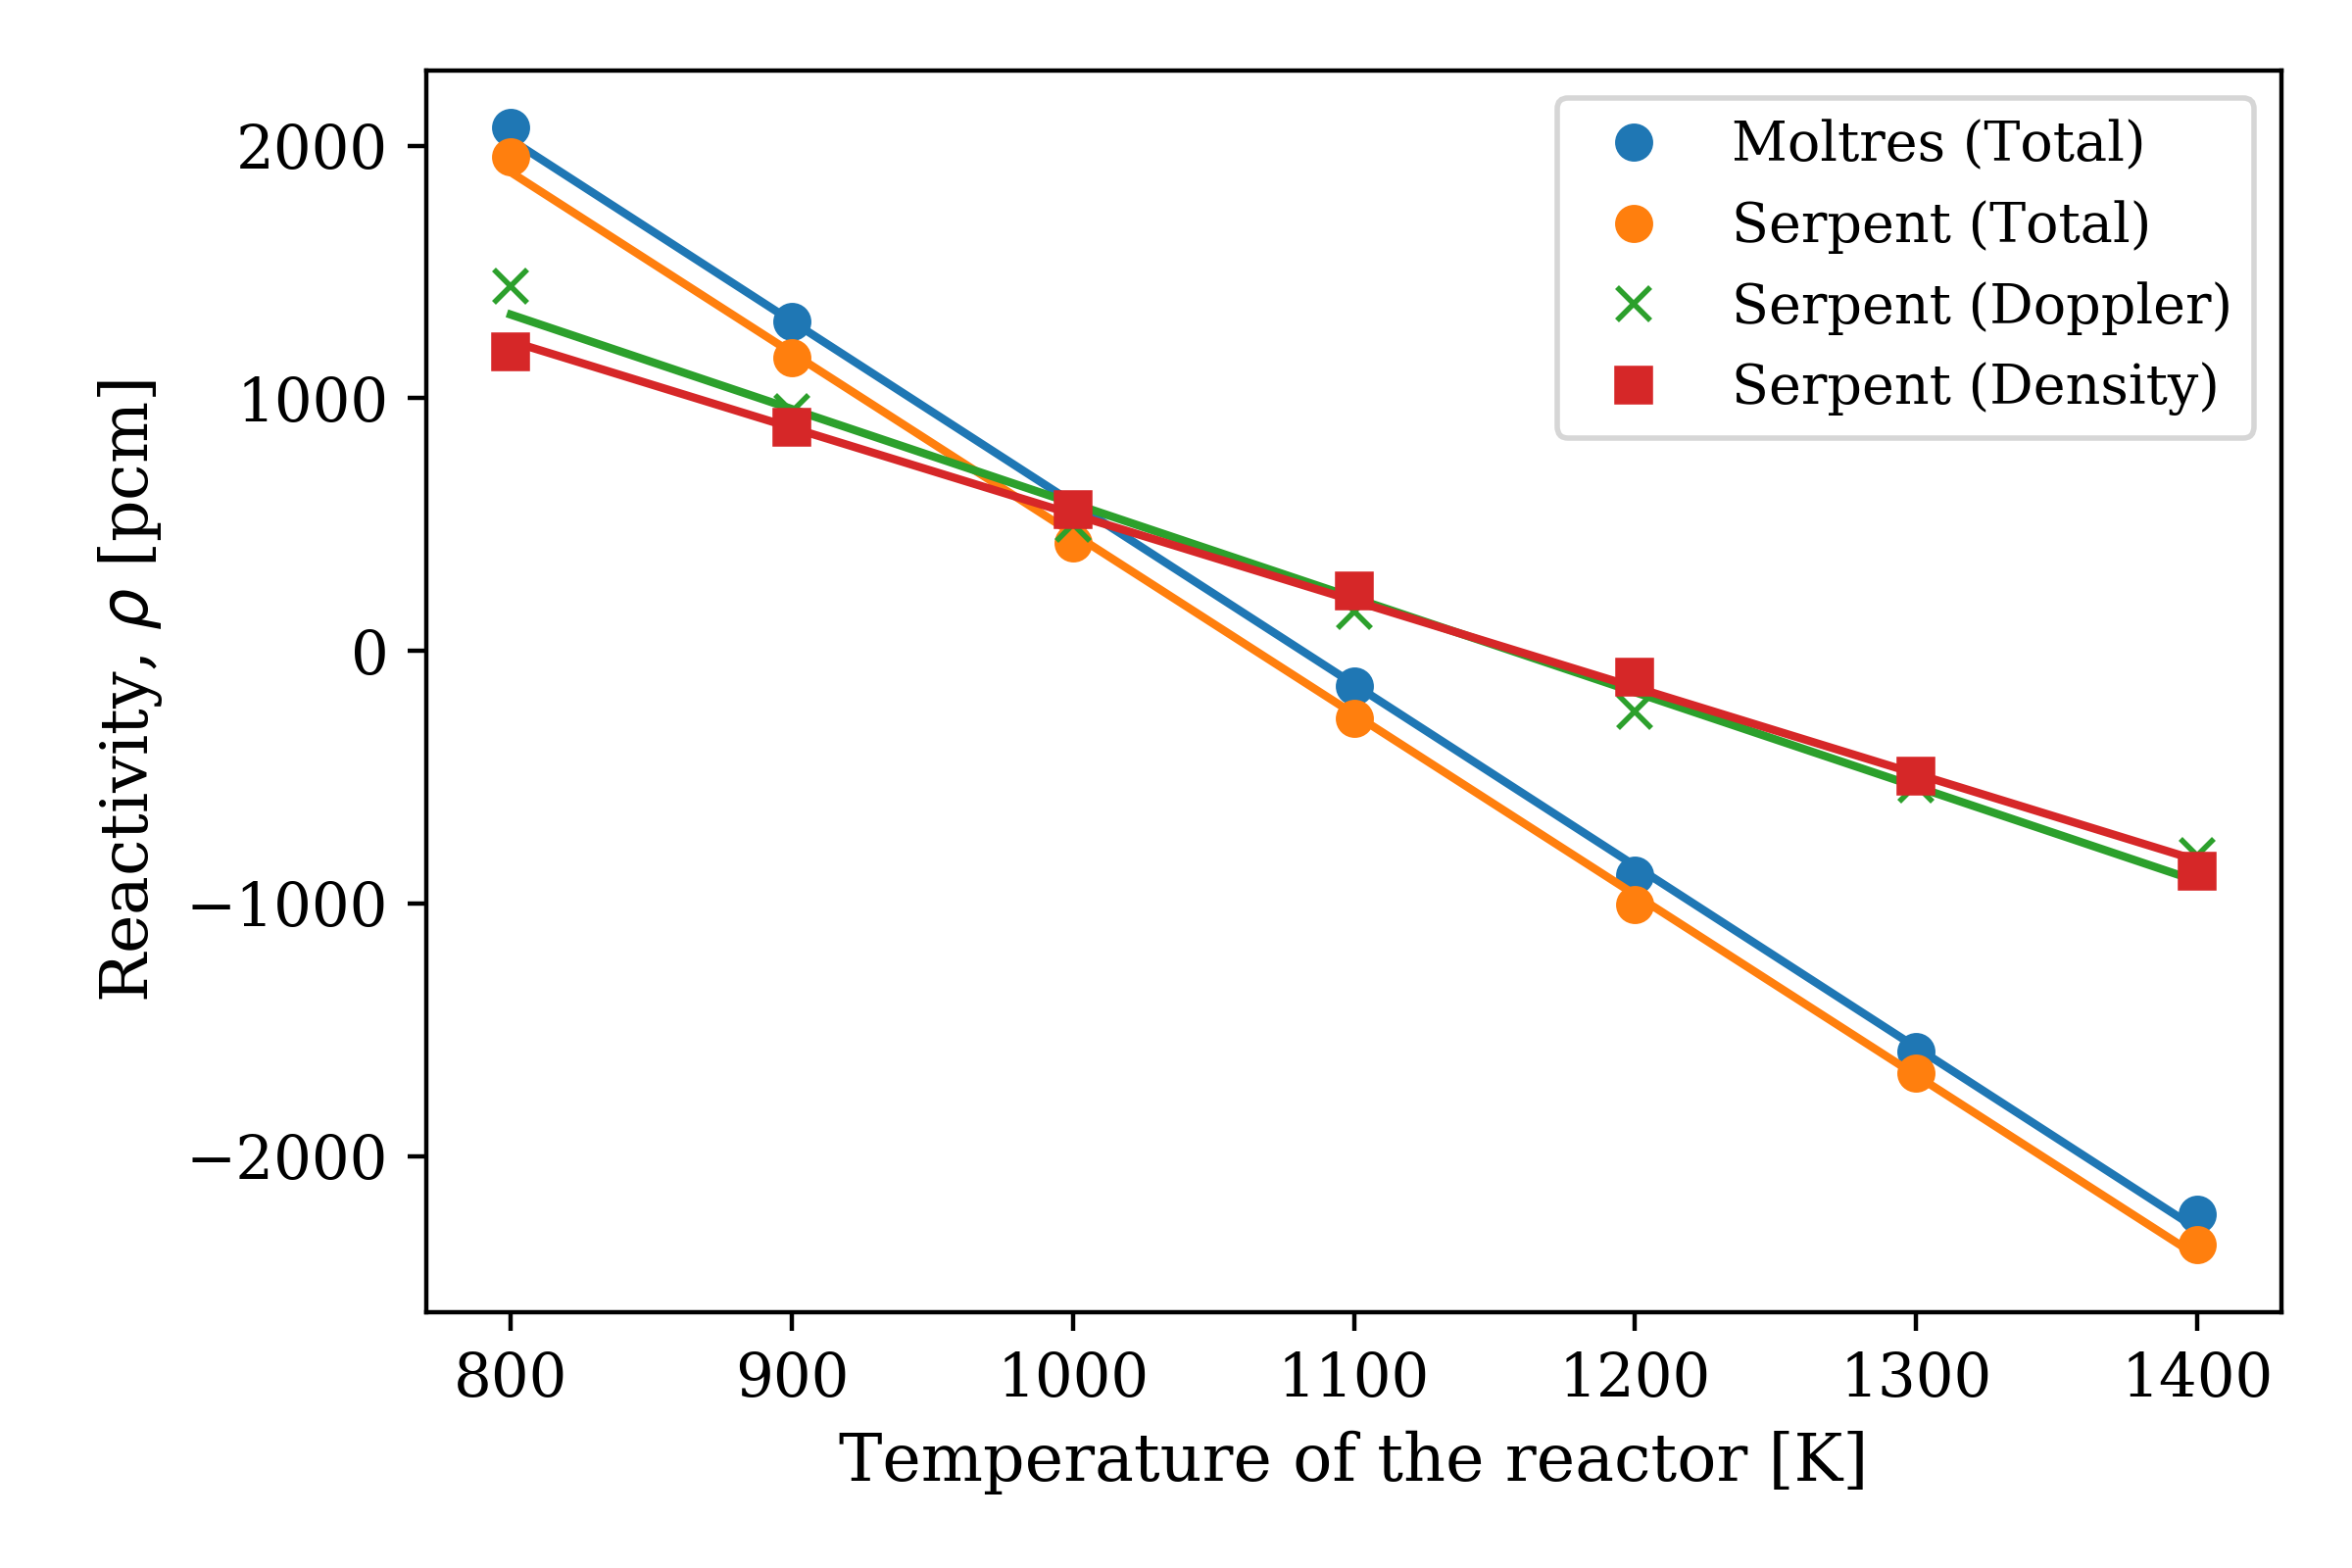
\includegraphics[width=.8\textwidth]{reactivity}
    \caption{Reactivity values from Serpent and Moltres. The Doppler
    reactivity values were calculated at a fixed density of 4.1249 g
    cm$^{-3}$. The thermal expansion reactivity values were calculated at a
    fixed temperature of 973 K.}
    \label{fig:reactivity}
\end{figure}
%
\begin{table}[htb!]
	\centering
	\caption{Doppler, density, and total temperature coefficients
	for the temperature range of 800 K to 1400 K.}
	\begin{tabular}{l S S S}
		\toprule
		{Software} & {$\alpha_D$ [pcm
		K$^{-1}$]} & {$\alpha_\rho$ [pcm K$^{-1}$]} & {$\alpha_T$ [pcm
		K$^{-1}$]} \\
		\midrule
		{Serpent} & -3.737 \pm 0.013 & -3.424 \pm 0.013 &
		-7.165 \pm 0.013 \\
		{Moltres} & {-} & {-} & -7.184\\
		\bottomrule
	\end{tabular}
	\label{table:alpha}
\end{table}

\section{Neutron Energy Spectrum}

\begin{figure}[htb!]
    \centering
    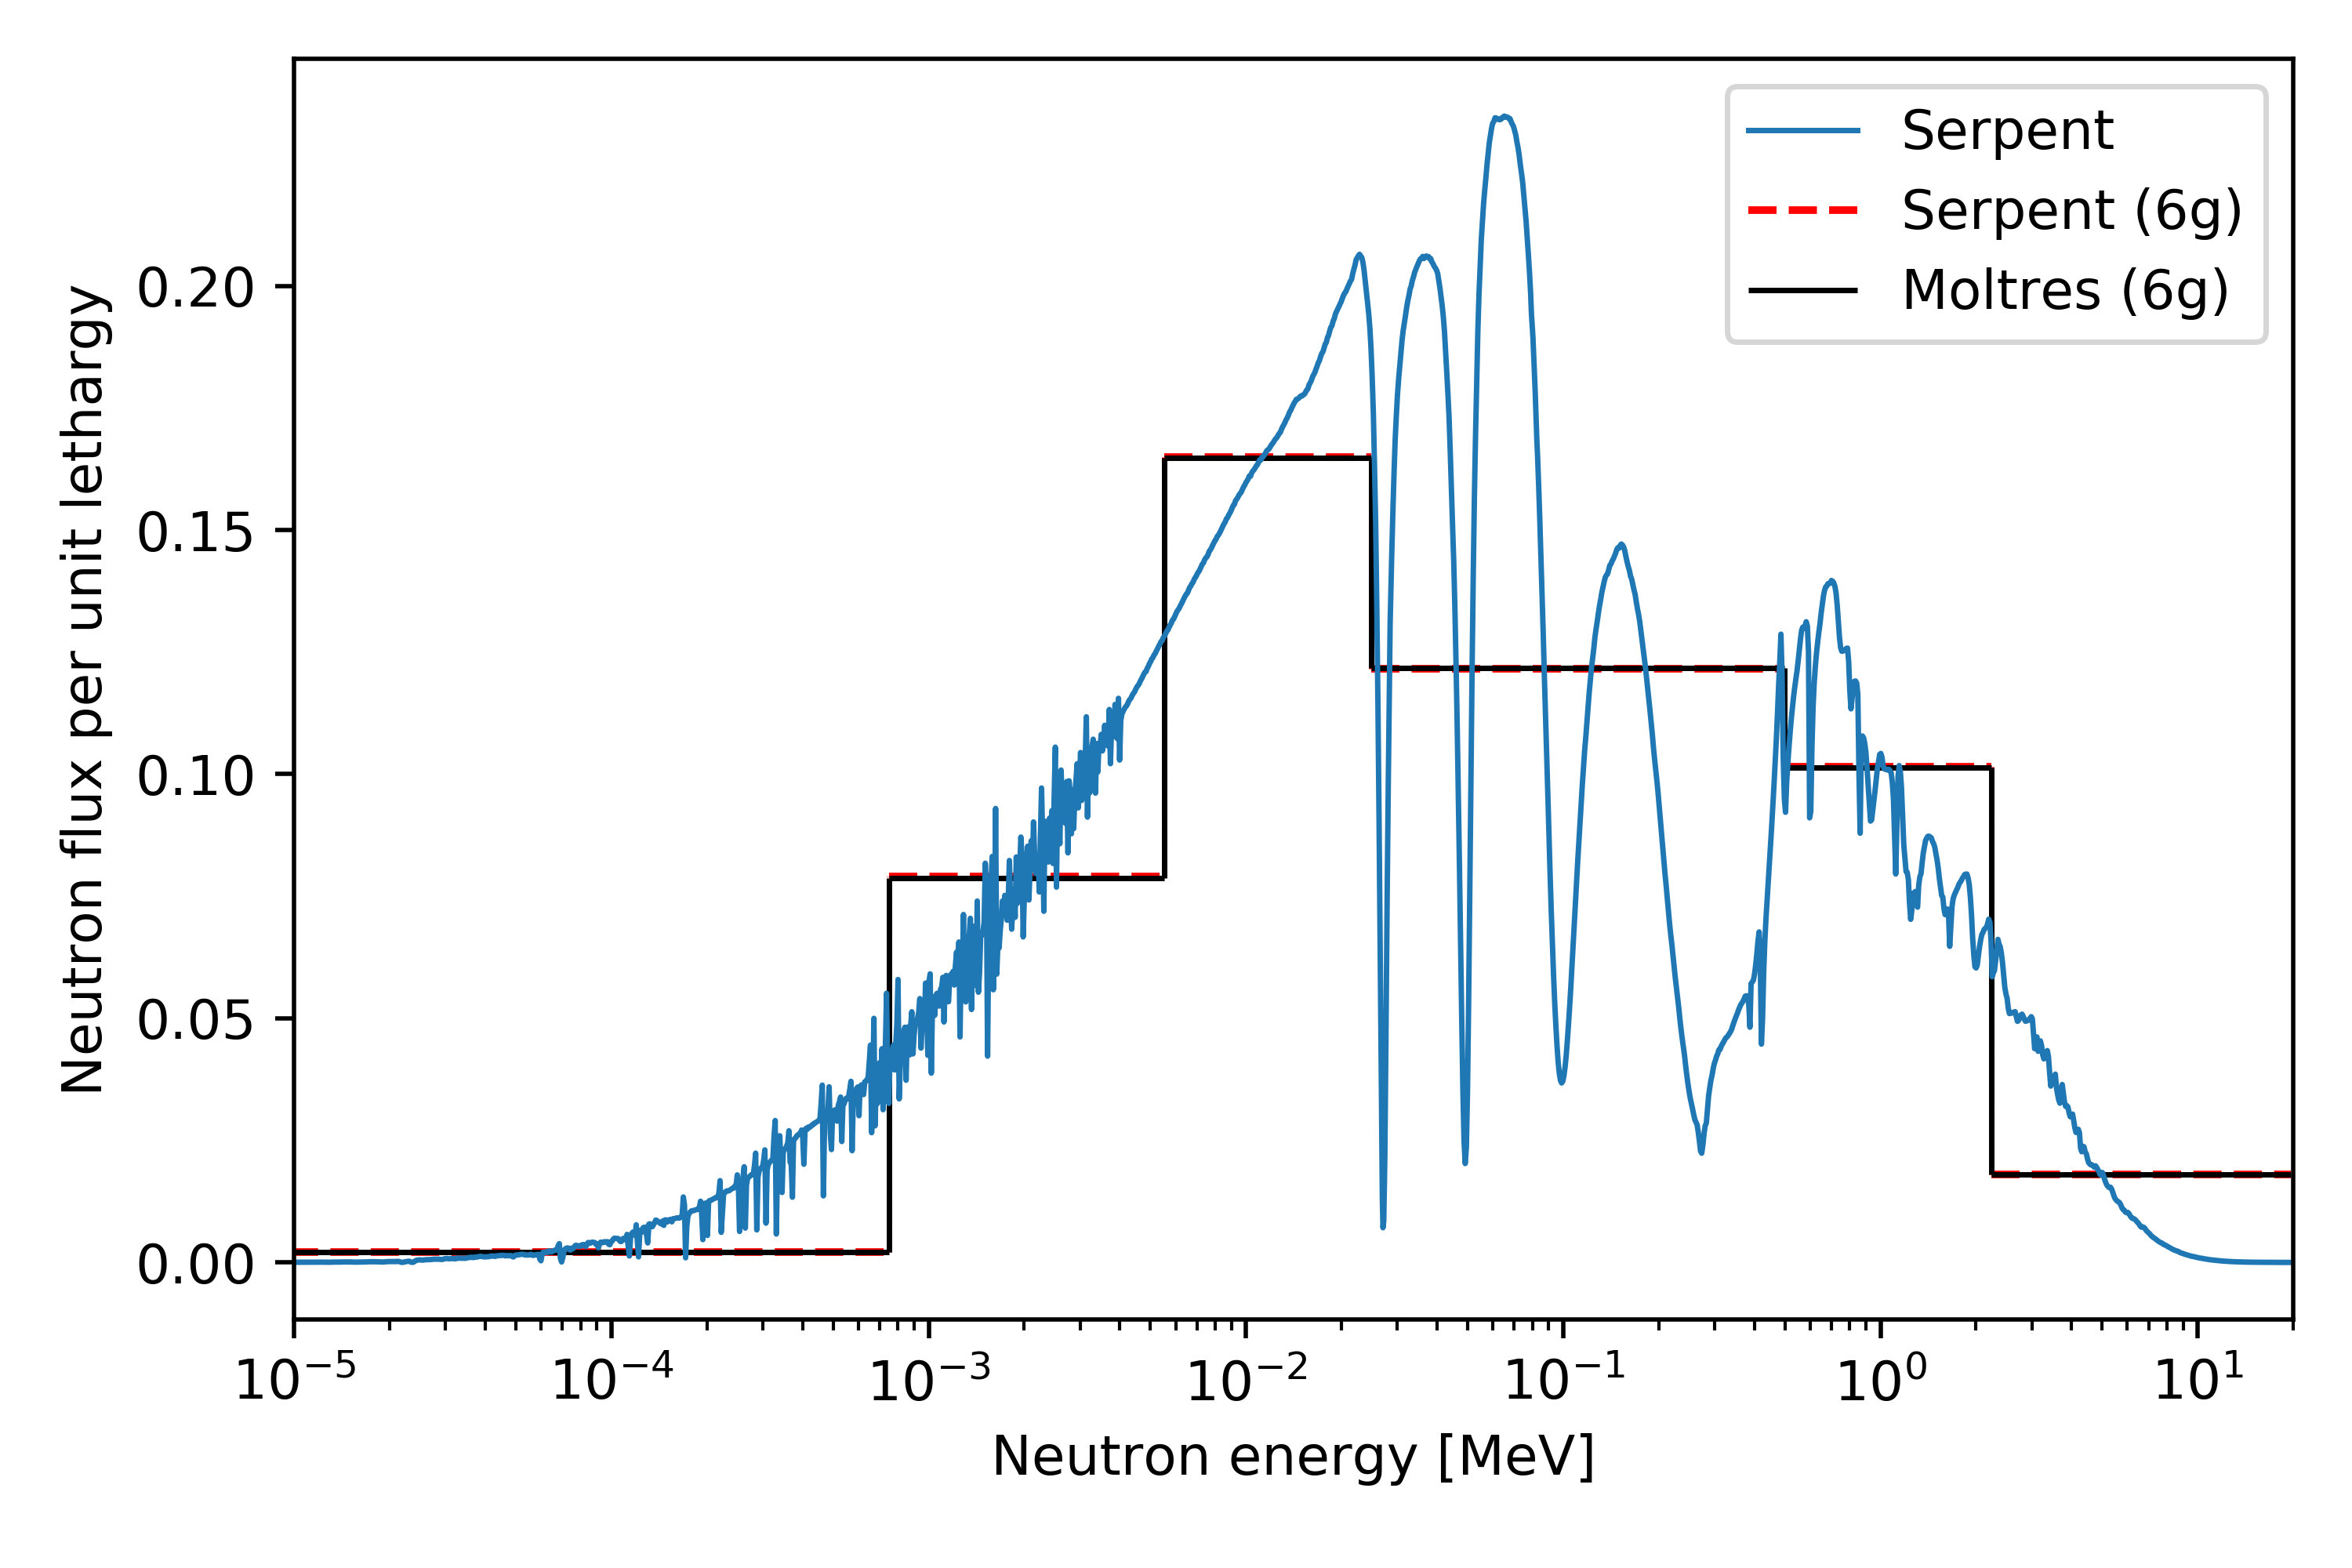
\includegraphics[width=.8\textwidth]{nt-spec}
    \caption{The fine-group and six-group neutron energy spectra from Serpent
    2 and Moltres normalized per unit lethargy.}
    \label{fig:ntspec}
\end{figure}

Moltres also closely replicated the six-group neutron spectrum from the
Serpent group constants. Figure \ref{fig:ntspec} compares the neutron energy
spectra from Serpent and Moltres in the central fuel salt region. More
generally, the
plot shows the distinctive fast spectrum observed in the \gls{MSFR} with dips
in the spectrum corresponding to elastic scattering resonances from lithium
and fluorine. We could obtain a more accurate representation of the neutronics
in the \gls{MSFR} by using more neutron energy groups with appropriate energy
boundaries but this would adversely impact simulation times in the
subsequent multiphysics finite element analyses.

In summary, Moltres replicated the relevant neutronics parameters
accurately using the group constant data from Serpent 2. Moltres agrees with
the high fidelity simulation in Serpent 2 for the $\beta_{\text{eff}}$ and
temperature reactivity coefficients, which are important parameters for
modeling transient reactor behavior. The $k_{\text{eff}}$ values have
discrepancies on the order of 100 pcm which are relatively small compared
to other \gls{MSR} multiphysics simulation tools (e.g. the neutron diffusion
and SP3 models in OpenFOAM \cite{cervi_development_2019}).
